\documentclass{article}

\usepackage{graphicx}
\usepackage{tikz}
\usepackage{tikzsymbols}
\usetikzlibrary{calc,patterns,shapes.geometric}
\pagestyle{empty}
\usepackage[margin=0pt]{geometry}
\geometry{papersize={14in,12in}}

\def\centerarc[#1](#2)(#3:#4:#5){\draw[#1] ($(#2)+({#5*cos(#3)},{#5*sin(#3)})$) arc (#3:#4:#5);}

\begin{document}
	\begin{figure}
		\centering
		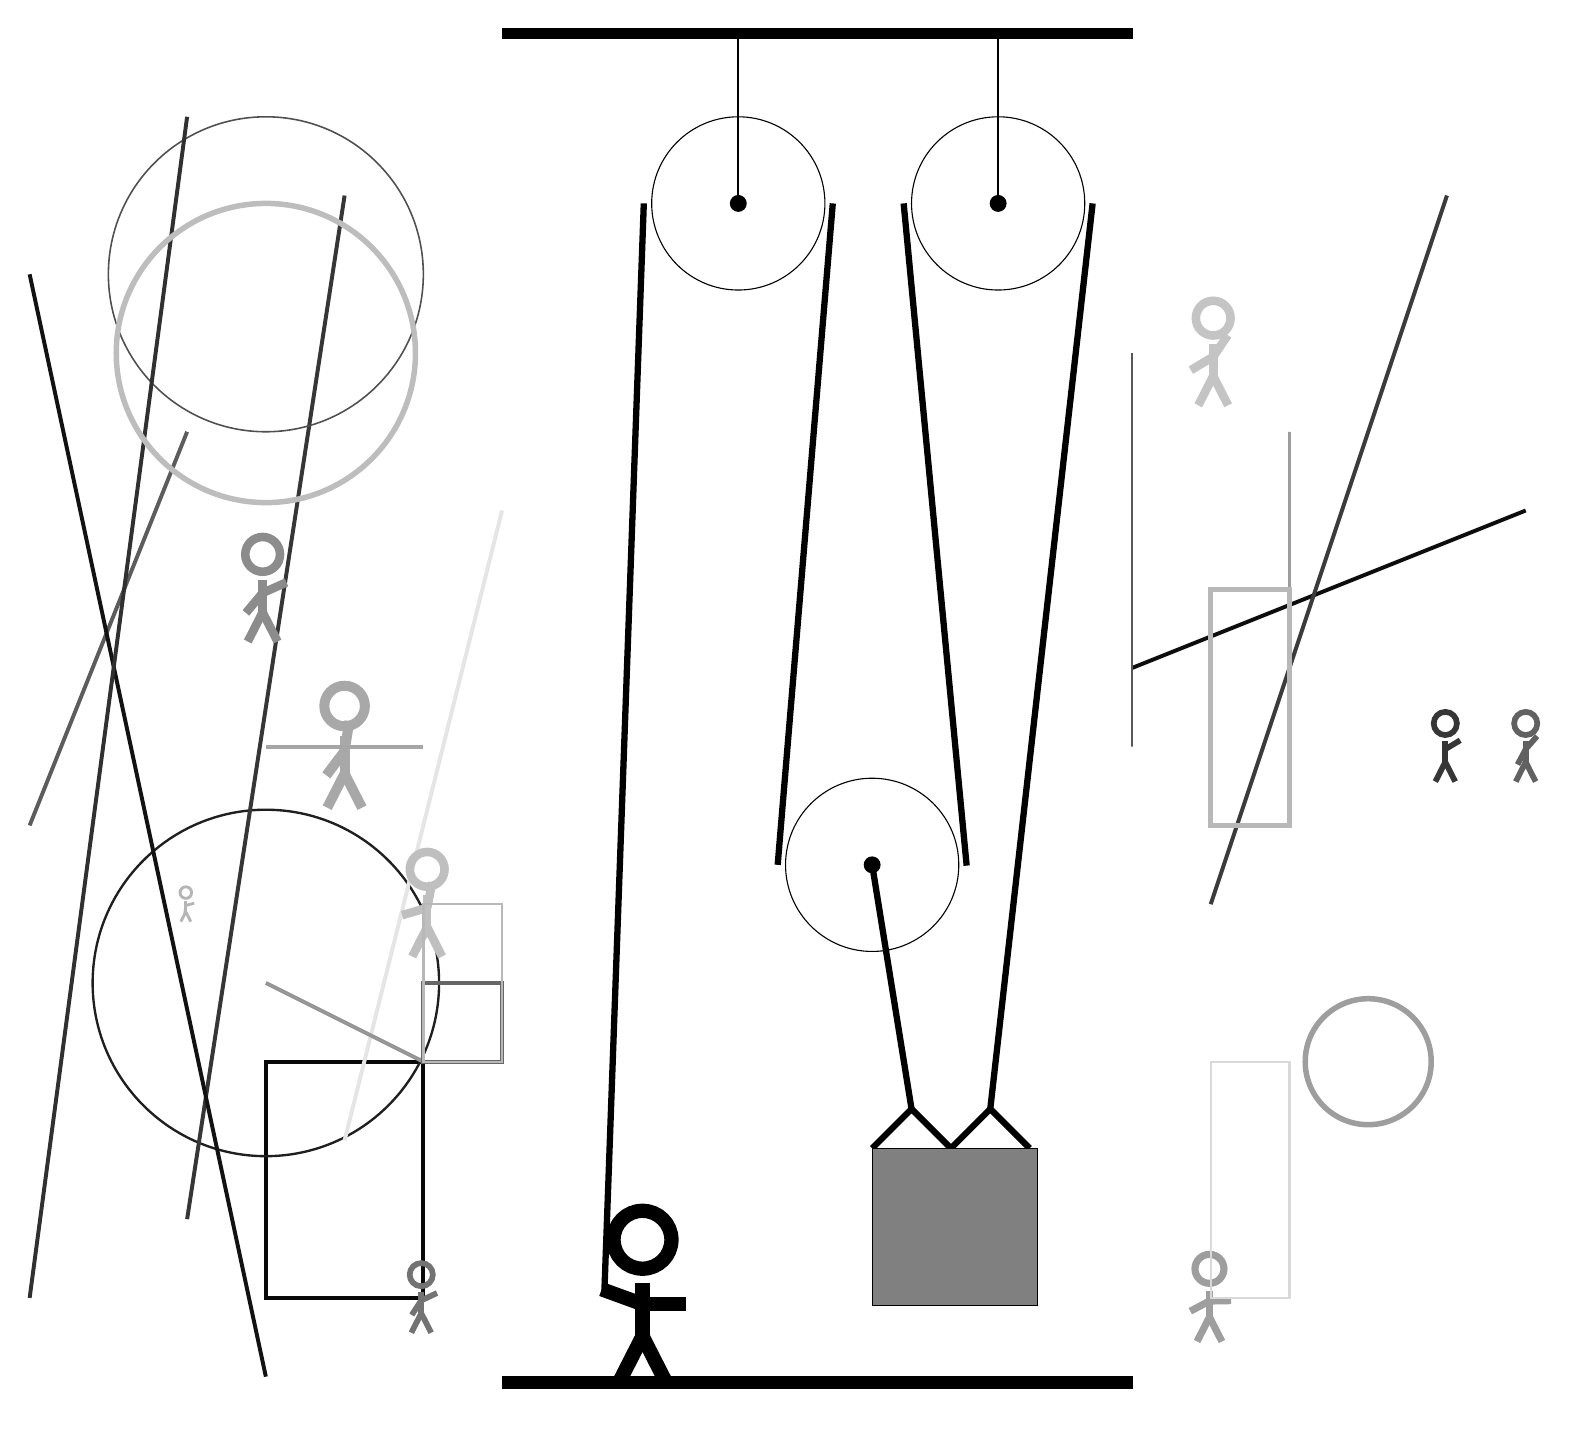
\begin{tikzpicture}
			%%%%% START %%%%%
			
			\draw[fill=black] (-2, 14) rectangle (6, 14.125);
			
			\node[line width=0.3mm, color=black!38] at (7, -2) {\Strichmaxerl[5][28][1]};
			
			\draw[line width=0.5mm, color=black!95](6, 6) -- (11, 8);
			\draw[line width=0.2mm, color=black!66] (6, 10) rectangle (6, 5);
			\draw[line width=0.5mm, color=black!39] (8, 9) rectangle (8, 7);
			\draw [line width=0.7mm, color=black!38](9, 1) circle (0.8);
			
			\draw[line width=0.5mm, color=black!97] (-3, -2) rectangle (-5, 1);
			\node[line width=0.2mm, color=black!34] at (-4, 5) {\Strichmaxerl[7][53][81]};
			\draw [line width=0.3mm, color=black!88](-5, 2) circle (2.2);
			\draw[line width=0.5mm, color=black!77](10, 12) -- (7, 3);
			\node[line width=0.7mm, color=black!55] at (-3, -2) {\Strichmaxerl[4][57][25]};
			\node[line width=0.6mm, color=black!23] at (7, 10) {\Strichmaxerl[6][31][56]};
			
			\draw[line width=0.5mm, color=black!64](-6, 9) -- (-8, 4);
			\draw[line width=0.5mm, color=black!79](-4, 12) -- (-6, -1);
			
			\node[line width=0.3mm, color=black!29] at (-6, 3) {\Strichmaxerl[2][83][15]};
			\draw[line width=0.5mm, color=black!10](-4, 0) -- (-2, 8);
			\draw[line width=0.5mm, color=black!93](-5, -3) -- (-8, 11);
			
			\draw[line width=0.5mm, color=black!35](-5, 5) -- (-3, 5);
			\node[line width=0.5mm, color=black!79] at (10, 5) {\Strichmaxerl[4][90][31]};
			\draw [line width=0.2mm, color=black!69](-5, 11) circle (2.0);
			
			\draw[line width=0.5mm, color=black!41](-5, 2) -- (-3, 1);
			\node[line width=0.4mm, color=black!25] at (-3, 3) {\Strichmaxerl[6][16][79]};
			
			\draw[line width=0.5mm, color=black!81](-6, 13) -- (-8, -2);
			\draw [line width=0.7mm, color=black!26](-5, 10) circle (1.9);
			\node[line width=0.5mm, color=black!45] at (-5, 7) {\Strichmaxerl[6][50][24]};
			\draw[line width=0.5mm, color=black!60] (-2, 1) rectangle (-3, 2);
			
			\node[line width=0.7mm, color=black!62] at (11, 5) {\Strichmaxerl[4][62][49]};
			\draw[line width=0.6mm, color=black!28] (7, 7) rectangle (8, 4);
			\draw[line width=0.3mm, color=black!28] (-2, 1) rectangle (-3, 3);
			\draw[line width=0.3mm, color=black!15] (7, -2) rectangle (8, 1);
			
			
			\draw (1, 11.9) circle (1.1);
			\draw[fill=black] (1, 11.9) circle (0.1);
			\draw[thick] (1, 11.9) -- (1, 14);
			
			\draw (4.3, 11.9) circle (1.1);
			\draw[fill=black] (4.3, 11.9) circle (0.1);
			\draw[thick] (4.3, 11.9) -- (4.3, 14);
			
			\draw (2.7, 3.5) circle (1.1);
			\draw[fill=black] (2.7, 3.5) circle (0.1);
			
			\draw[line width=0.8mm]  (2.7, -0.1) -- (3.2, 0.4) -- (3.7, -0.1) -- (4.2, 0.4) -- (4.7, -0.1);
			\draw[fill=black!50] (2.7, -0.1) rectangle (4.8, -2.1);
			
			\draw[line width=0.8mm](-0.7, -1.9) -- (-0.2, 11.9);
			\centerarc[line width=0.8mm](1, 11.9)(0:180:1.2000000000000002);
			\draw[line width=0.8mm](2.2, 11.9) -- (1.5, 3.5);
			\centerarc[line width=0.8mm](2.7, 3.5)(180:370:1.2000000000000002);
			\draw[line width=0.8mm] (3.9, 3.49) -- (3.1, 11.9);
			\centerarc[line width=0.8mm](4.3, 11.9)(0:180:1.2000000000000002);
			\draw[line width=0.8mm](4.2, 0.4) -- (5.5, 11.9);
			\draw[line width=0.8mm] (3.2, 0.4) -- (2.7, 3.5);
			
			\node at (-0.2, -2) {\Strichmaxerl[10][-20][0]};
			
			\draw[fill=black] (-2, -3) rectangle (6, -3.15);
			
			%%%%% END %%%%%
		\end{tikzpicture}
	\end{figure}	
\end{document}